\documentclass{article}
\usepackage{braket}
\usepackage{amsmath}
\usepackage{MnSymbol}
\usepackage{graphicx}
\newcommand{\bfit}[1]{\textbf{\textit{#1}}}
\begin{document}
\textbf{\large 4.5 Basic Quantum Gatess}
\\\\
In this section, we will first review the directions and properties of some basic
quantum gates and their matrix form. Readers may refer to chapters 15 to 18 in [1]
for more detailed discussions.

It should be noted that (1) all quantum gates are defined based on how they
transform the basis states, (2) every quantum gate has a corresponding matrix once the basis is 
chosen, and (3) all quantum gates must be \textbf{unitary} as discussed in Sect. 4.4.
\\\\
\textbf{\textit{\large 4.5.1 Identity Gate}}
\\\\
The \textbf{identity gate}, \textbf{\textit{I}}, as its name implies, keeps a 
vector unchanged. In physics, applying an identity gate to a state
means leaving the state as it it without applying any interaction
(\textbf{\textit{H}} is zero matrix in Eq.(4.1)). While it weems that it is 
trivial and redundant, it plays an important role when one needs to construct an operator for
a large space formed by a tensor product of smaller ones, in which on qubit goes
through a non-trivial operator and one qubit is left unchanged.

An identity gate is defines as,
\begin{align} \label{eq 4.33}
    \begin{split}
        \textbf{\textit{I}}\ket{0} = \ket{0},\\
        \textbf{\textit{I}}\ket{1} = \ket{1}.\\
    \end{split} \tag{4.33}
\end{align}

Therefore, when it is applied to a negeral state $\ket{\psi} = \alpha\ket{0}+\beta\ket{1}$,
we have,
\begin{align} \label{eq 4.34}
    \begin{split}
         \textbf{\textit{I}}\ket{\psi} &=\textbf{\textit{I}}(\alpha\ket{0}+\beta\ket{1}), \\
        &= \textbf{\textit{I}}\alpha\ket{0}+\textbf{\textit{I}}\beta\ket{1}, \\
         &= \alpha\textbf{\textit{I}}\ket{0}+\beta\textbf{\textit{I}}\ket{1}, \\
        &= \aleph\ket{0}+ \beta\ket{1},\\
        &= \ket{\psi}.
    \end{split} \tag{4.34}
\end{align}
The matrix of \textit{\textbf{I}} is
\begin{equation} \label{eq 4.35}
    \textbf{\textit{I}}=\begin{pmatrix}
        1 \ 0\\0 \ 1
    \end{pmatrix}.\tag{4.35}
\end{equation}

\textit{\textbf{\large 4.5.2 NOT Gate}}\\\\
The \textbf{NOT} gate, \textbf{\textit{U}}$_{NOT}$, is defined as,
\begin{align} \label{eq 4.36}
    \begin{split}
        \textbf{\textit{U}}_{\textit{\textbf{NOT}}}\ket{0}=\ket{1},\\
        \textbf{\textit{U}}_{\textit{\textbf{NOT}}}\ket{1}=\ket{0}.
    \end{split} \tag{4.36}
\end{align}

Therefore, when it is applied to a negeral state $\ket{\psi}=\alpha\ket{0}+\beta\ket{1}$, we have,
\begin{align} \label{eq 4.37}
    \begin{split}
        textbf{\textit{U}}_{\textit{\textbf{NOT}}}\ket{\psi}&=\textbf{\textit{U}}_{\textit{\textbf{NOT}}}(\alpha\ket{0})+\beta\ket{1}),\\
        &= \alpha\textbf{\textit{U}}_{\textit{\textbf{NOT}}}\ket{0}+\beta\textbf{\textit{U}}_{\textit{\textbf{NOT}}}\ket{1},\\
        &= \alpha\ket{0}+\beta\ket{1}.
    \end{split} \tag{4.37}
\end{align}
The matrix \textbf{\textit{U}}$_{\textit{\textbf{NOT}}}$ is
\begin{equation} \label{eq 4.38}
    \textbf{\textit{U}}_{\textit{\textbf{NOT}}}=\begin{pmatrix}
        0\ 1 \\ 1\ 0
    \end{pmatrix}.\tag{4.38}
\end{equation}

\textit{\textbf{\large 4.5.3 Phase Shift Gate}}\\\\
A \textbf{phsse shift gate}, \textbf{\textit{U}}$_{\boldsymbol{PS,\varPhi}}$, 
has a \textbf{gate parameter}, $\boldsymbol{\varPhi}$. This parameter detemines how much 
\textit{relative} phase shift will be applied to a qunatum state.
A phase shift gate is defined as,
\begin{align} \label{eq 4.39}
    \begin{split}
        \textit{\textbf{U}}_{\boldsymbol{PS,\varPhi}}\ket{0}&=\ket{0},\\
        \textit{\textbf{U}}_{\boldsymbol{PS,\varPhi}}\ket{1}&=e^{i\varPhi}\ket{1}.
    \end{split} \tag{4.39}
\end{align}

Therefore, when it is applied to a genral state $\ket{\psi}=\alpha\ket{0}+\beta\ket{1}$,
we have,
\begin{align} \label{eq 4.40}
    \begin{split}
         \textit{\textbf{U}}_{\boldsymbol{PS,\varPhi}}\ket{\psi}&=  \textit{\textbf{U}}_{\boldsymbol{PS,\varPhi}}(\alpha\ket{0}+\beta\ket{1}),\\
         &=\alpha \textit{\textbf{U}}_{\boldsymbol{PS,\varPhi}}\ket{0}+\beta \textit{\textbf{U}}_{\boldsymbol{PS,\varPhi}}\ket{1},\\
         &=\alpha\ket{0}+\beta e^{i \varPhi}\ket{1}.
    \end{split}\tag{4.40}
\end{align}
The matrix of  $\textit{\textbf{U}}_{\boldsymbol{PS,\varPhi}}\ket{0}$ is
\begin{equation} \label{eq 4.41}
     \textit{\textbf{U}}_{\boldsymbol{PS,\varPhi}}\ket{0}=\begin{pmatrix}
        1& 0\\0& e^{i\varPhi}
     \end{pmatrix}.\tag{4.41}
\end{equation}

If we set $\varPhi$ to $\pi, \pi/2$, and $\pi/4$, we will obtain \textit{\textbf{Z, S}} and \textit{\textbf{T}} gates, respectively.
That is,
\begin{equation} \label{eq 4.42}
\textit{\textbf{Z}}=\begin{pmatrix}
    1& 0\\0& e^{i\pi}
\end{pmatrix}= \begin{pmatrix}
    1& 0\\0& -1
\end{pmatrix}. \tag{4.42}
\end{equation}\\
\begin{equation} \label{eq 4.43}
    \textit{\textbf{S}}=\begin{pmatrix}
    1& 0\\0& e^{i\frac{\pi}{2}}
\end{pmatrix}= \begin{pmatrix}
    1& 0\\0& i
\end{pmatrix}. \tag{4.43}
\end{equation}\\
\begin{equation} \label{eq 4.44}
    \textit{\textbf{T}}=\begin{pmatrix}
    1& 0\\0& e^{i\frac{\pi}{4}}
\end{pmatrix}.\tag{4.44}
\end{equation}
It is important to recognize that $\textit{\textbf{U}}_{\boldsymbol{PS,\varPhi}}$ only
changes the \textbf{relative phase} between the coefficients of the tow basis
states, $\ket{0}$ and $\ket{1}$. It does \textit{not} change the square of the modulus
of the coefficients because $|e^{i\varPhi}|=1$. Therefore, it does not
change the probability of the state collapsing to each basis state (see Eqs. (2.21) and (2.22)).
\\\\
\bfit{\large 4.5.4 Hadamard Gate}\\\\
The \textbf{Hadamard gate}, \bfit{H}, is a qunatum gate to create
\textbf{superposition}. Although I am using the same symbol as the Hamiltonian,
we should not be confused. A Hadamard gate is define as, 
\begin{align} \label{eq 4.45}
    \begin{split}
        \bfit{H}\ket{0}&=\frac{1}{\sqrt{2}}(\ket{0}+\ket{1})=\ket{+},\\
        \bfit{H}\ket{1}&=\frac{1}{\sqrt{2}}(\ket{0}1\ket{1})=\ket{-},
    \end{split}\tag{4.45    }
\end{align}
where we have dfined $\ket{+}=\frac{1}{\sqrt{2}}(\ket{0}+\ket{1})$ and
$\ket{-}=\frac{1}{\sqrt{2}}(\ket{0}-\ket{1})$.

Therefore, when it is applied to a general state $\ket{\psi}=\alpha\ket{0}+\beta\ket{1}$,
we have,
\begin{align} \label{eq 4.46}
    \begin{split}
        \bfit{H}\ket{\psi}&=\bfit{H}(\alpha\ket{0}+\beta\ket{1}),\\
        &= \alpha\bfit{H}\ket{0}+\beta\bfit{H}\ket{1},\\
        &=\alpha\ket{+}+\beta\ket{-}.
    \end{split} \tag{4.46}
\end{align}
The matrix of \bfit{H} is
\begin{equation} \label{eq 4.47}
    \bfit{I}=\frac{1}{\sqrt{2}}\begin{pmatrix}
        1 &1\\1 & -1
    \end{pmatrix}. \tag{4.47}
\end{equation}
It should be noted that \bfit{H} equals its inverse \bfit{H$^{-1}$}; therefore,
\begin{equation} \label{eq 4.48}
    \bfit{H}\bfit{H}=\bfit{H}\bfit{H}^{\bfit{-1}}=\bfit{I}. \tag{4.48}
\end{equation}
\\\\
\bfit{\large 4.5.5 CNOT gate}
\\\\
The \textbf{CNOT} gate, \bfit{U}$_{\bfit{X\! O\! R}}$, is also called the \textbf{XOR} gate. CNOT
stands for \textbf{controlled NOT}. It is a 2-qubit gate. This means that it is 
4 $\times$ 4 matrix. The Hamiltonian used to generate the gate (see Eq. (4.31)) is also a 4 $\times$ 4
matrix in the 4D space with basis states $\ket{00}, \ket{01}, \ket{10},$ and $\ket{11}$
(see Sect. 2.4). A CNOT gate has one \textbf{control qubit} and one \textbf{target qubit}.
Their meanings can be understood better by first looking at the definition
of \bfit{U}$_{\bfit{X\! O\! R}}$,
\begin{align} \label{eq 4.49}
    \begin{split}
        \bfit{U}_{\bfit{X\! O\! R}}\ket{00}=\ket{0\oplus0,0}=\ket{0,0}=\ket{00},\\
        \bfit{U}_{\bfit{X\! O\! R}}\ket{01}=\ket{0\oplus1,1}=\ket{0,1}=\ket{01},\\
        \bfit{U}_{\bfit{X\! O\! R}}\ket{10}=\ket{1\oplus1,0}=\ket{1,1}=\ket{11},\\
        \bfit{U}_{\bfit{X\! O\! R}}\ket{11}=\ket{1\oplus1,1}=\ket{1,0}=\ket{10},\\
    \end{split} \tag{4.49}
\end{align}
which can be summarized as
\begin{equation} \label{eq 4.50}
    \bfit{U}_{\bfit{X\! O\! R}}\ket{ab}=\ket{a,a\oplus b},\tag{4.50}
\end{equation}
with \textit{a} and \textit{b} taking the value of 0 or 1.$\oplus$ is the \textit{classical}
XOR operation, which explains why this gate is also called and XOR gate.
We can also understand its definition from a "control-target" point of view.
When it is applied to a basis \textit{ket}, if the \textbf{most significant bit (MSB)}
is 0 in the \textit{ket}, the \textbf{least significant bit (LSB)} is unchange.
If the MSB is 1 in the \textbf{ket}, the LSB is flipped which is equivalent to
having received a \textit{classical} NOT operation. Therefore, the MSB is a control qubit,
the LSB is a target qubit, and the operation is a controlled-NOT operation. 
When it is applied to a general state $\ket{\psi}=\alpha\ket{00}+\beta\ket{01}+\gamma\ket{10}+\delta\ket{11}$,
we have,
\begin{align} \label{eq 4.51}
    \begin{split}
        \bfit{U}_{\bfit{X\! O\! R}}\ket{\psi}&=\bfit{U}_{\bfit{X\! O\! R}}(\alpha\ket{00}+\beta\ket{01}+\gamma\ket{10}+\delta\ket{11}),\\
        &= \alpha\bfit{U}_{\bfit{X\! O\! R}}\ket{00}+\beta\bfit{U}_{\bfit{X\! O\! R}}\ket{01}+\gamma\bfit{U}_{\bfit{X\! O\! R}}\ket{10}+\delta\bfit{U}_{\bfit{X\! O\! R}}\ket{11},\\
        &= \alpha\ket{00}+\beta\ket{01}+\gamma\ket{11}+\delta\ket{10},\\
        &= \alpha\ket{00}+\beta\ket{01}+\delta\ket{10}+\gamma\ket{11},\\
    \end{split}\tag{4.51}
\end{align}
which can be visualized in the top circuit in Fig. 4.1.

The matrix of $\bfit{U}_{\bfit{X\! O\! R}}$ is
\begin{equation}
    \bfit{U}_{\bfit{X\! O\! R}}=\begin{pmatrix}
        1\ 0\ 0\ 0\\0\ 1\ 0\ 0\\0\ 0\ 0\ 1\\0\ 0\ 1\ 0
    \end{pmatrix}. \tag{4.52}
\end{equation}

We may also swap the role of the MSB and LSB such that the LSB is the
control qubit and the MSB is the target qubit (the bottom circuit in Fig. 4.1).
In this case, we have
\begin{align} \label{eq 4.53}
    \begin{split}
       \bfit{U}_{\bfit{X\! O\! R}}\ket{00}=\ket{0\oplus0,0}=\ket{0,0}=\ket{00},\\
        \bfit{U}_{\bfit{X\! O\! R}}\ket{01}=\ket{0\oplus1,1}=\ket{1,1}=\ket{11},\\
        \bfit{U}_{\bfit{X\! O\! R}}\ket{10}=\ket{1\oplus0,0}=\ket{1,0}=\ket{10},\\
        \bfit{U}_{\bfit{X\! O\! R}}\ket{11}=\ket{1\oplus1,1}=\ket{0,1}=\ket{01},\\
    \end{split}\tag{4.53}
\end{align}
\\\\
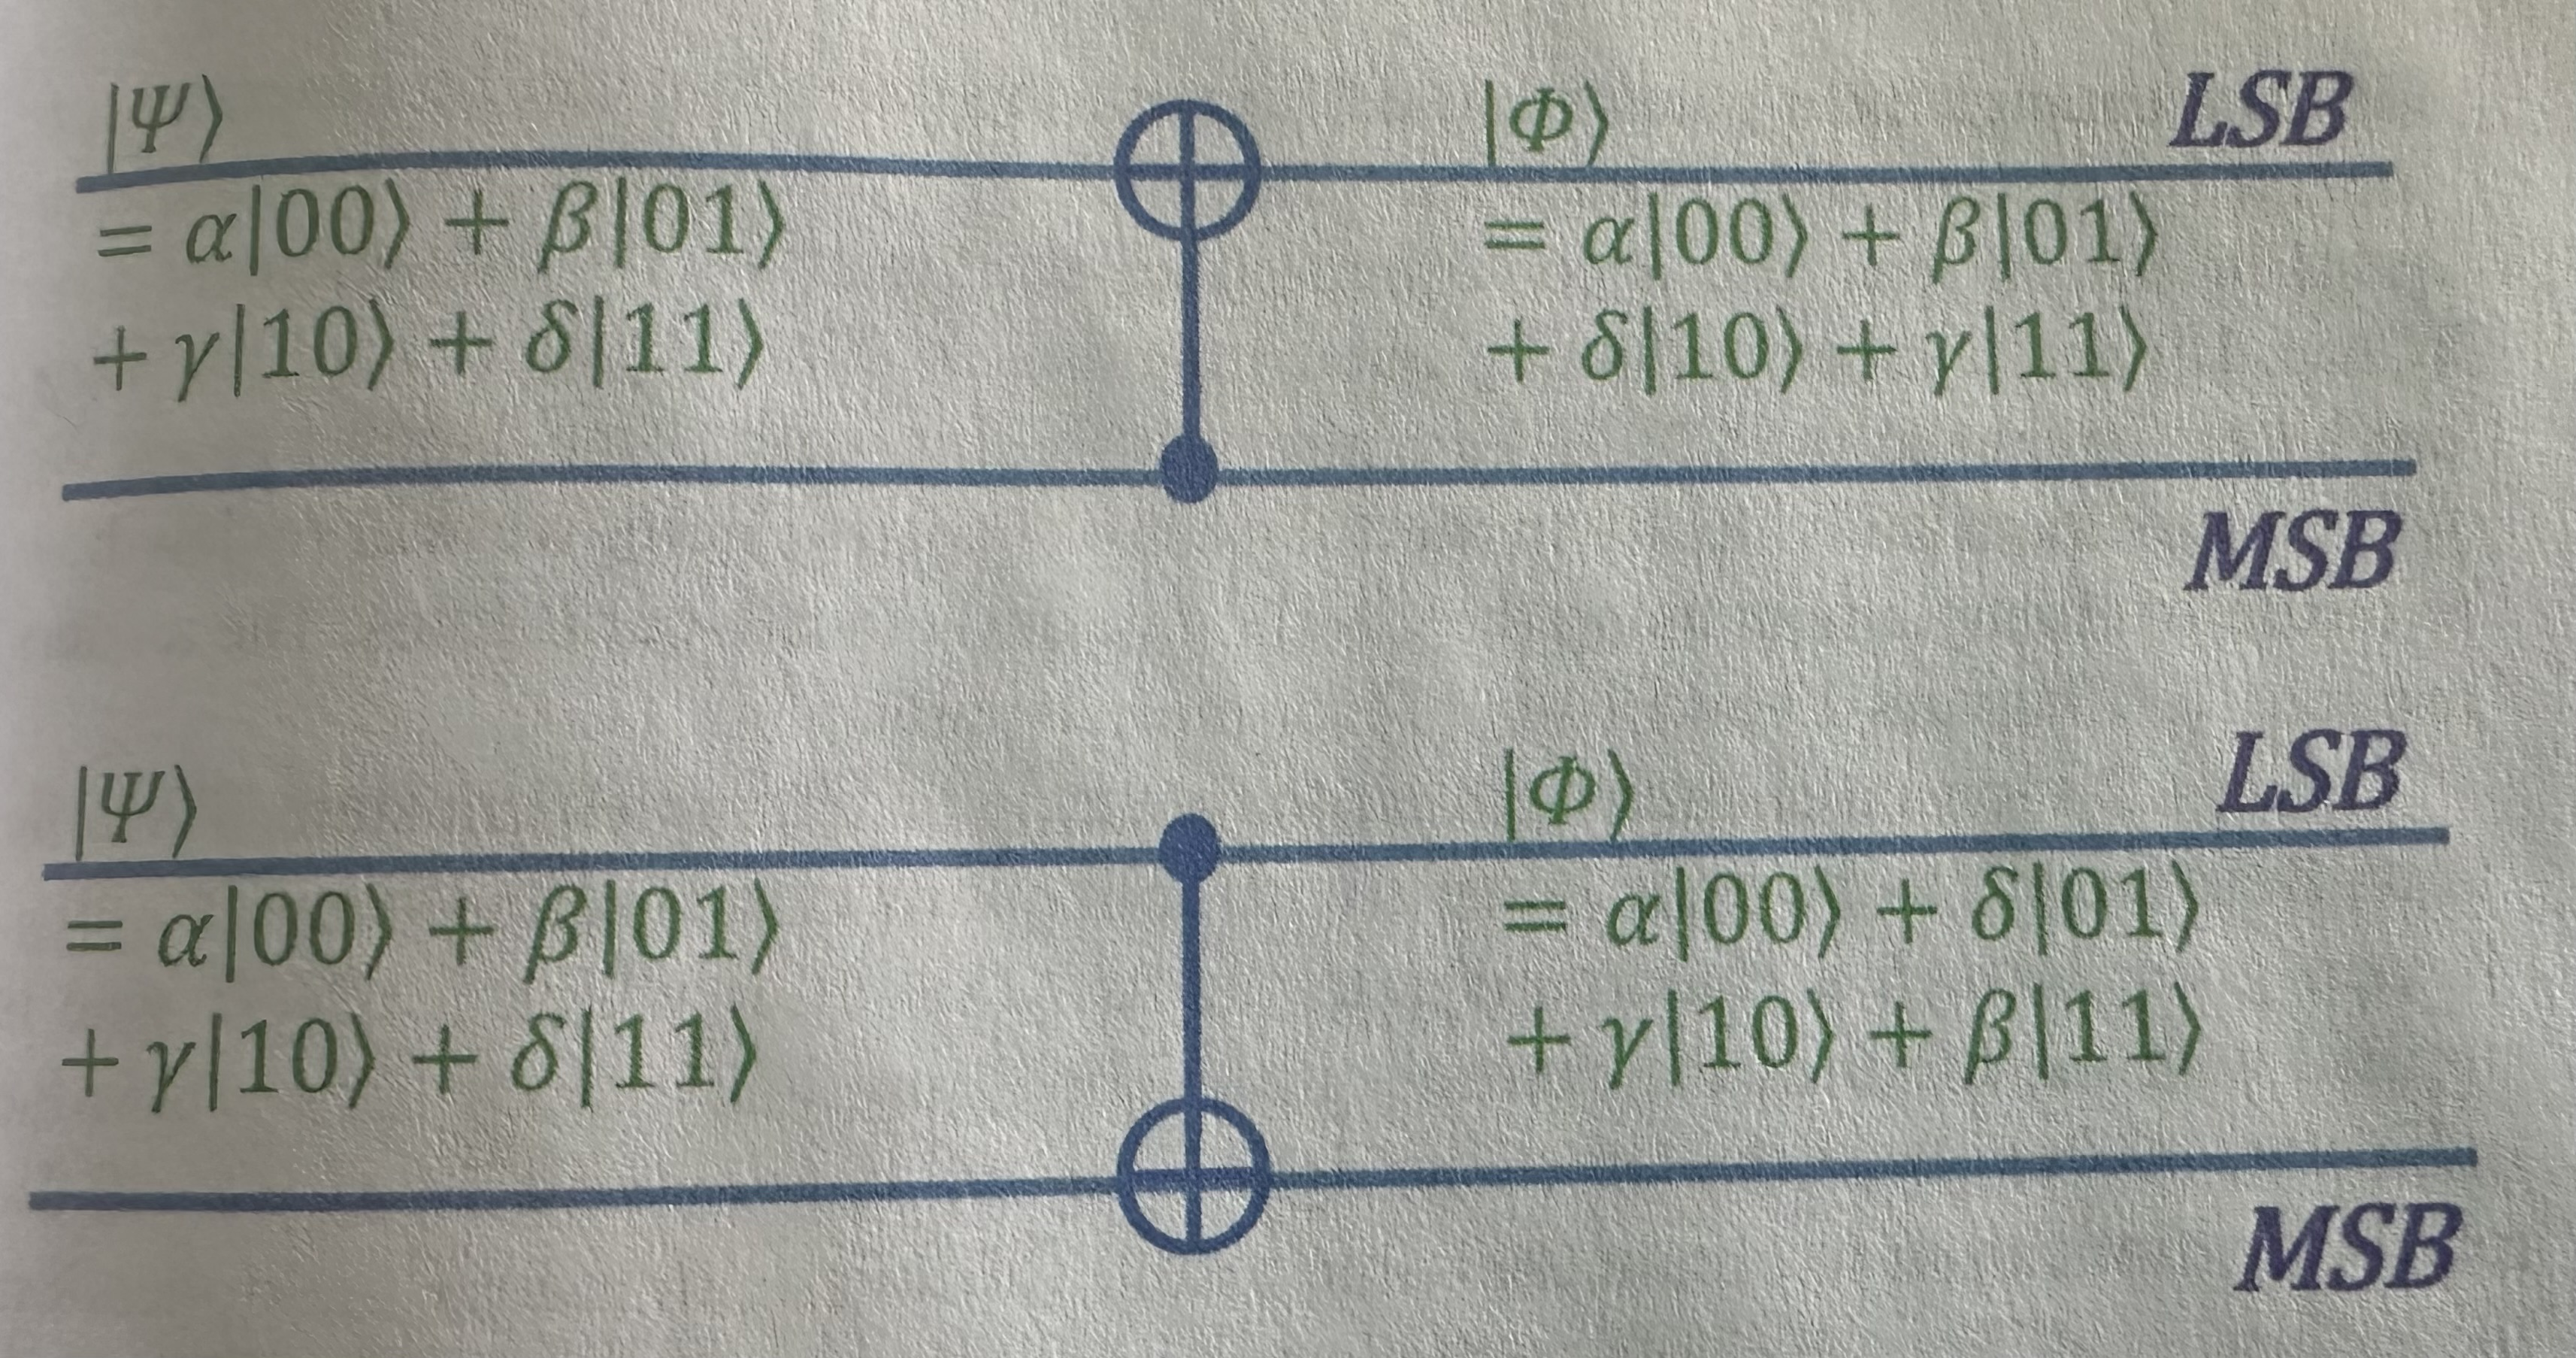
\includegraphics[scale=0.4]{Fig 4.1.jpeg}\\
\textbf{Fig. 4.1} Operation of a CNOT gate. Top: the MSB is the control qubit.
Bottom: the LSB is the control qubit
\\\\
Therfore,
\begin{align}\label{eq 4.54}
    \begin{split}
         \bfit{U}_{\bfit{X\! O\! R}}\ket{\psi}&=\bfit{U}_{\bfit{X\! O\! R}}(\alpha\ket{00}+\beta\ket{01}+\gamma\ket{10}+\delta\ket{11}),\\
        &= \alpha\bfit{U}_{\bfit{X\! O\! R}}\ket{00}+\beta\bfit{U}_{\bfit{X\! O\! R}}\ket{01}+\gamma\bfit{U}_{\bfit{X\! O\! R}}\ket{10}+\delta\bfit{U}_{\bfit{X\! O\! R}}\ket{11},\\
        &= \alpha\ket{00}+\beta\ket{11}+\gamma\ket{10}+\delta\ket{01},\\
        &= \alpha\ket{00}+\delta\ket{01}+\gamma\ket{10}+\beta\ket{11},\\ 
    \end{split} \tag{4.54}
\end{align}
and,
\begin{equation}
    \bfit{U}_{\bfit{X\! O\! R}}=\begin{pmatrix}
        1\ 0\ 0\ 0\\0\ 0\ 0\ 1\\0\ 0\ 1\ 0\\0\ 1\ 0\ 0
    \end{pmatrix}. \tag{4.55}
\end{equation}
\\\\
\textbf{\large 4.6 Engtanglement}
\\\\
\textbf{Entanglement}, in addition to superposition, is what makes quantum computing
powerful. A CNOT gate is an entanglement gate that can be used to create
entangled states. In any quantum hardware, we need to be able to implement at least
one entnaglement gate. Other commonly used entanglement gates are controlled-phase shift gates
and iSWAP gates. For different quantum computing architectures,different entanglement gates
are used because the gates that can be generated are limited by the available Hamiltonian (Eq. (4.31)).
For example, an electron spin qubit in silicon may use a controlled-phase shift gate as its entanglement
gate  (Chap. 12) and a superconducting qubit may use an iSWAP gate (Caph. 21).
They are all equivalent to the CNOT gate after combining with some 1-qubit gates.
We will discuss them individually in teh following chapters. Here, we will review how
to create an entanglement using the CNOT gate and other 1-qubit gates.
The readers can refer to Chapters 13 and 14 in [1] for more details.

Figure 4.2 shows a quantum circuit for creating an entanglement state. The time flows
from  the left to the right. It starts with both qubits at the ground state $\ket{0}_A \ket{0}_B$.
It then goes throught a Hadamard gate for its MSB after which a CNOT gate is applied
with the MSB as the control qubit. The figure has already shown how the
qubit state evolves from the left to the right using bra-ket notation. Here, we will use
matrix multiplication to obtain the same result. Of course, in matrix multiplication,
the process goes from the right to the left in the \textit{equation}. The output is
\begin{align} \label{eq 4.56}
    \begin{split}
        &\bfit{U}_{\bfit{X\! O\! R}}(\bfit{H}\otimes\bfit{I})\ket{00},\\
        =&\begin{pmatrix}
            1\ 0\ 0\ 0\\ 0\ 1\ 0\ 0\\ 0\ 0\ 0\ 1\\0\ 0\ 1\ 0
        \end{pmatrix}\frac{1}{\sqrt{2}}
        \begin{pmatrix}
            1& 1\\ 1& -1
        \end{pmatrix}\otimes
        \begin{pmatrix}
            1\ 0\\ 0\ 1
        \end{pmatrix}
        \begin{pmatrix}
            1\\0\\0\\0
        \end{pmatrix},\\
        =&\begin{pmatrix}
            1\ 0\ 0\ 0\\ 0\ 1\ 0\ 0\\ 0\ 0\ 0\ 1\\0\ 0\ 1\ 0
        \end{pmatrix}\frac{1}{\sqrt{2}}
        \begin{pmatrix}
            1& 0& 1& 0\\0& 1& 0& 1\\1& 0& -1& 0\\0& 1& 0& -1
        \end{pmatrix}
        \begin{pmatrix}
            1\\0\\0\\0
        \end{pmatrix},\\
        =&\begin{pmatrix}
            1\ 0\ 0\ 0\\ 0\ 1\ 0\ 0\\ 0\ 0\ 0\ 1\\0\ 0\ 1\ 0
        \end{pmatrix}\frac{1}{\sqrt{2}}
        \begin{pmatrix}
            1\\0\\1\\0
        \end{pmatrix},\\
        =&\frac{1}{\sqrt{2}}\begin{pmatrix}
            1\\0\\0\\1
        \end{pmatrix},\\
        =&\frac{1}{\sqrt{2}}(\ket{00}+\ket{11}),
    \end{split}\tag{4.56}
\end{align}
resulting in an entangled state.\\\\
\textbf{\large 4.7 Summary}
\\\\
We learn how to solve the Schr\"{o}dinger equation using matrix formulation.
We need to be careful when performing matrix expotential when the matrix is non-diagonal.
We show that the Hamiltonian and the time Hamiltonian is applied would
determine the effective quantum gate. Therefore, the creation of quantum gate is 
nothing but \textbf{Hamiltonian engineering}. We review some of the fundamental 
1- qubit gates. We also reveiw the CNOT gate which can be used to create entanglement.
It is important to note that the control qubit can be either the MSB or LSB.
Finally, the CNOT gate might not be the native entanglement gate in some technologies.
However, it is equivalent to them after combining with some 1-qubit quantum gates and we will
discuss them in the following chapters.

\textbf{\large Problems}\\\\
\textbf{4.1 The Schr\"{o}dinger Equation}

Show that Eqs. (4.12) and (4.13) are the solutions of Eqs. (4.10) and (4.11), respectively.
\\\\
\textbf{4.2 Matrix Expotential through Diagonalization}

Find e$^{-i\frac{H}{\hbar}t}$ for the \bfit{H} in Eqs. (4.23) by first diagonalizing \bfit{H}.
Then calculate the matrix exponential in the diagonal form. Using the transformation matrix to convert
it back to the origianl basis. Note that you need to find the eigenvectors in this process.
You will find that two of the eigenvalues are 0 and you want to pick the two
corresponding eigenvectors to be orthonormal to others.
\\\\
\textbf{4.3 Phase Shift Gates}

Using matrix multiplication, show that $\bfit{T}^4=\bfit{S}^2=Z$.
\\\\
\textbf{4.4 Entanglement Circuit}

Create an entanglement circuit and use matrix multiplication to prove
the function of the circuit when the control qubit is the LSB.
\\\\
\textbf{References}
\\\\
1. Hiu-Yung Wong. \textit{Introduction to Quantum computing}. Springer, 2024.
2. J.J. Sakurai. \textit{Modern Quantum Mechanics}. Addison-Wesley, 1993.
\end{document}